\svnid{$Id$}
\chapter{Nitric Oxide Reduction in \Nm{}}
\label{chap:noreduction}
\section{Aerobic Nitric Oxide Reduction}
\subsection{Introduction}
The next dataset used in the iterative approach to parameter estimation was of aerobic oxygen reduction interrupted by the addition of Nitric Oxide. These datasets are the next most complicated after aerobic oxygen reduction as it introduces the nitric oxide reduction pathway. In this case the oxygen reduction and Nitric Oxide reduction pathways are active. Additionally, inactivation of \cbbthree{} by Nitric Oxide was occurring. The portions of the ETC relating to Nitric Oxide reduction are shown graphically in Figure \ref{fig:no_resp_chain}. However this pathway cannot be isolated \textit{in vivo} as \Nm{} is incapable of completely anaerobic respiration therefore the required parts of the model are actually those from Chapter \ref{chap:oxygenreduction} and those in Figure \ref{fig:no_resp_chain}.
\begin{figure}[tbp]
  \centering
    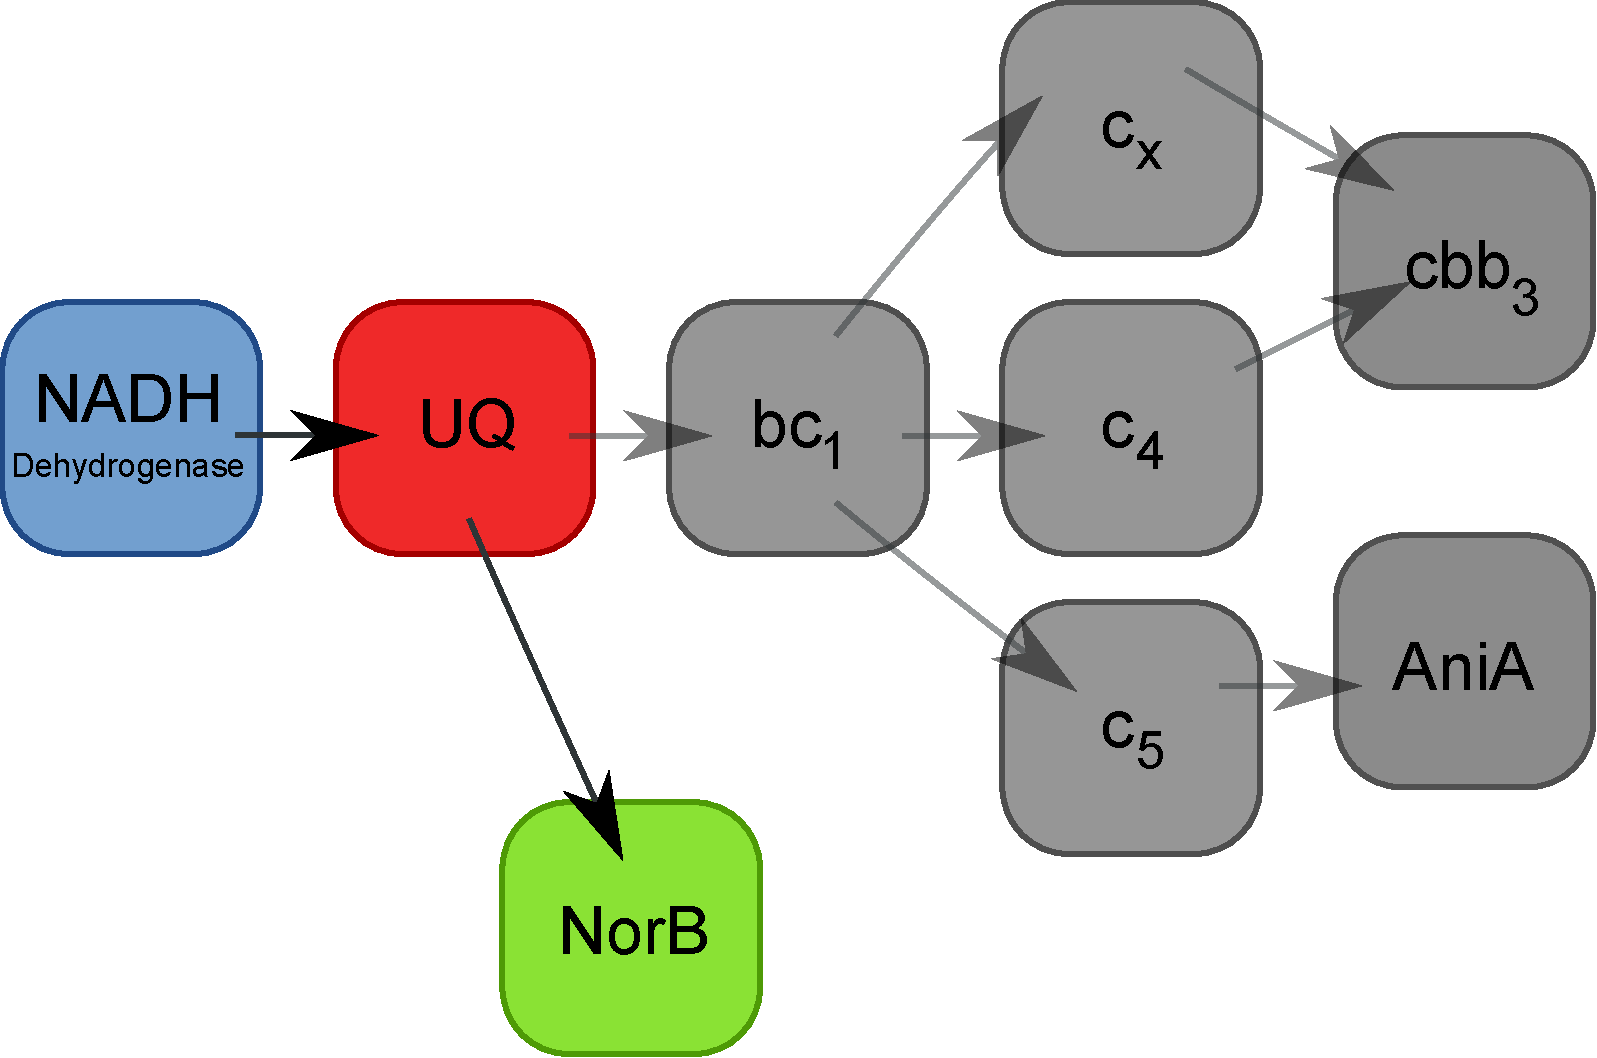
\includegraphics[width=14cm]{06-noreduction/data/no_resp_chain.pdf}
    \caption[Nitric oxide reducing electron transport chain of \Nm{}]{{\bf Nitric oxide reducing electron transport chain of \Nm{}.} This shows the complete electron transport chain of \Nsm{} with the components irrelevant to nitric oxide reduction greyed out.
  \label{fig:no_resp_chain}}
\end{figure}\\
The equations that describe this portion of the ETC are:
\begin{eqnarray*}
\frac{d[O_2]}{dt} & = & \beta(1-[O_2]/K_O) - k_{1}[C_a][O_2]\\
\frac{d[Q_a]}{dt} & = & g([Q] - [Q_a]) - l_3[Q_a]([B] - [B_a]) - f[Q_a]([X]-[X_a])\\
\frac{d[X_a]}{dt} & = & -k_3([C] - [C_a] - [C_X])[X_a]  - m_3([A] - [A_a])[X_a] + f[Q_a]([X]-[X_a])\\
\frac{d[C_a]}{dt} & = & k_3([C] - [C_a] - [C_X])[X_a] - k_{1}[C_a][O_2] - k_5[C_a][NO] + k_6[C_X]\\
\frac{d[NO]}{dt} & = & m_{1}[NO_2^-][A_a] - l_1[NO][B_a] - k_5[C_a][NO] + k_6 [C_X] - \gamma[NO]\\
\frac{d[C_X]}{dt} & = & k_5[C_a][NO] - k_6 [C_X]\\
\frac{d[B_a]}{dt} & = & l_3[Q_a]([B] - [B_a]) - l_1[NO][B_a]
\end{eqnarray*}
These equations describe the change in concentration of Nitric Oxide over time, which is the experimentally observable value (in addition to the afore modelled oxygen). Also being modelled was the change in concentration of inhibited \cbbthree{} and the reduction state of NorB. This more complete portion of the model involved 24 parameters and variables which were to be estimated. This number includes the 13 values already estimated in Chapter \ref{chap:oxygenreduction}.
\subsection{Experimental Results}
Generation of Nitric Oxide reduction datasets required the growth of MC58 (wild type \Nsm{}) in aerobic conditions until mid log-phase growth had been achieved. This corresponds to an $OD_{600}$ of 0.3-0.9 and usually required an incubation period of roughly 3 hours. Once the required cell density had been obtained, the culture was transferred to the oxygen electrode chamber and the oxygen and nitric oxide concentrations recorded as the culture respired. To model nitric oxide reduction required that nitric oxide solution was added to the culture while it is respiring aerobically. Part-way through aerobic respiration nitric oxide solution was added to various final concentrations all at $\approx 5~\mu$M and the culture then left to reduce nitric oxide (in addition to oxygen). The nitric oxide reduction datasets generated and used for parametrisation of this portion of the model are shown in Figures \ref{fig:nodata}, \ref{fig:nodata1} \& \ref{fig:nodata2}. Unfortunately the experimental data upon addition of nitric oxide is very difficult to reliably reproduce, with different cultures having apparently different tolerances to nitric oxide (data not shown).

\begin{figure}[tbp]
 \centering
 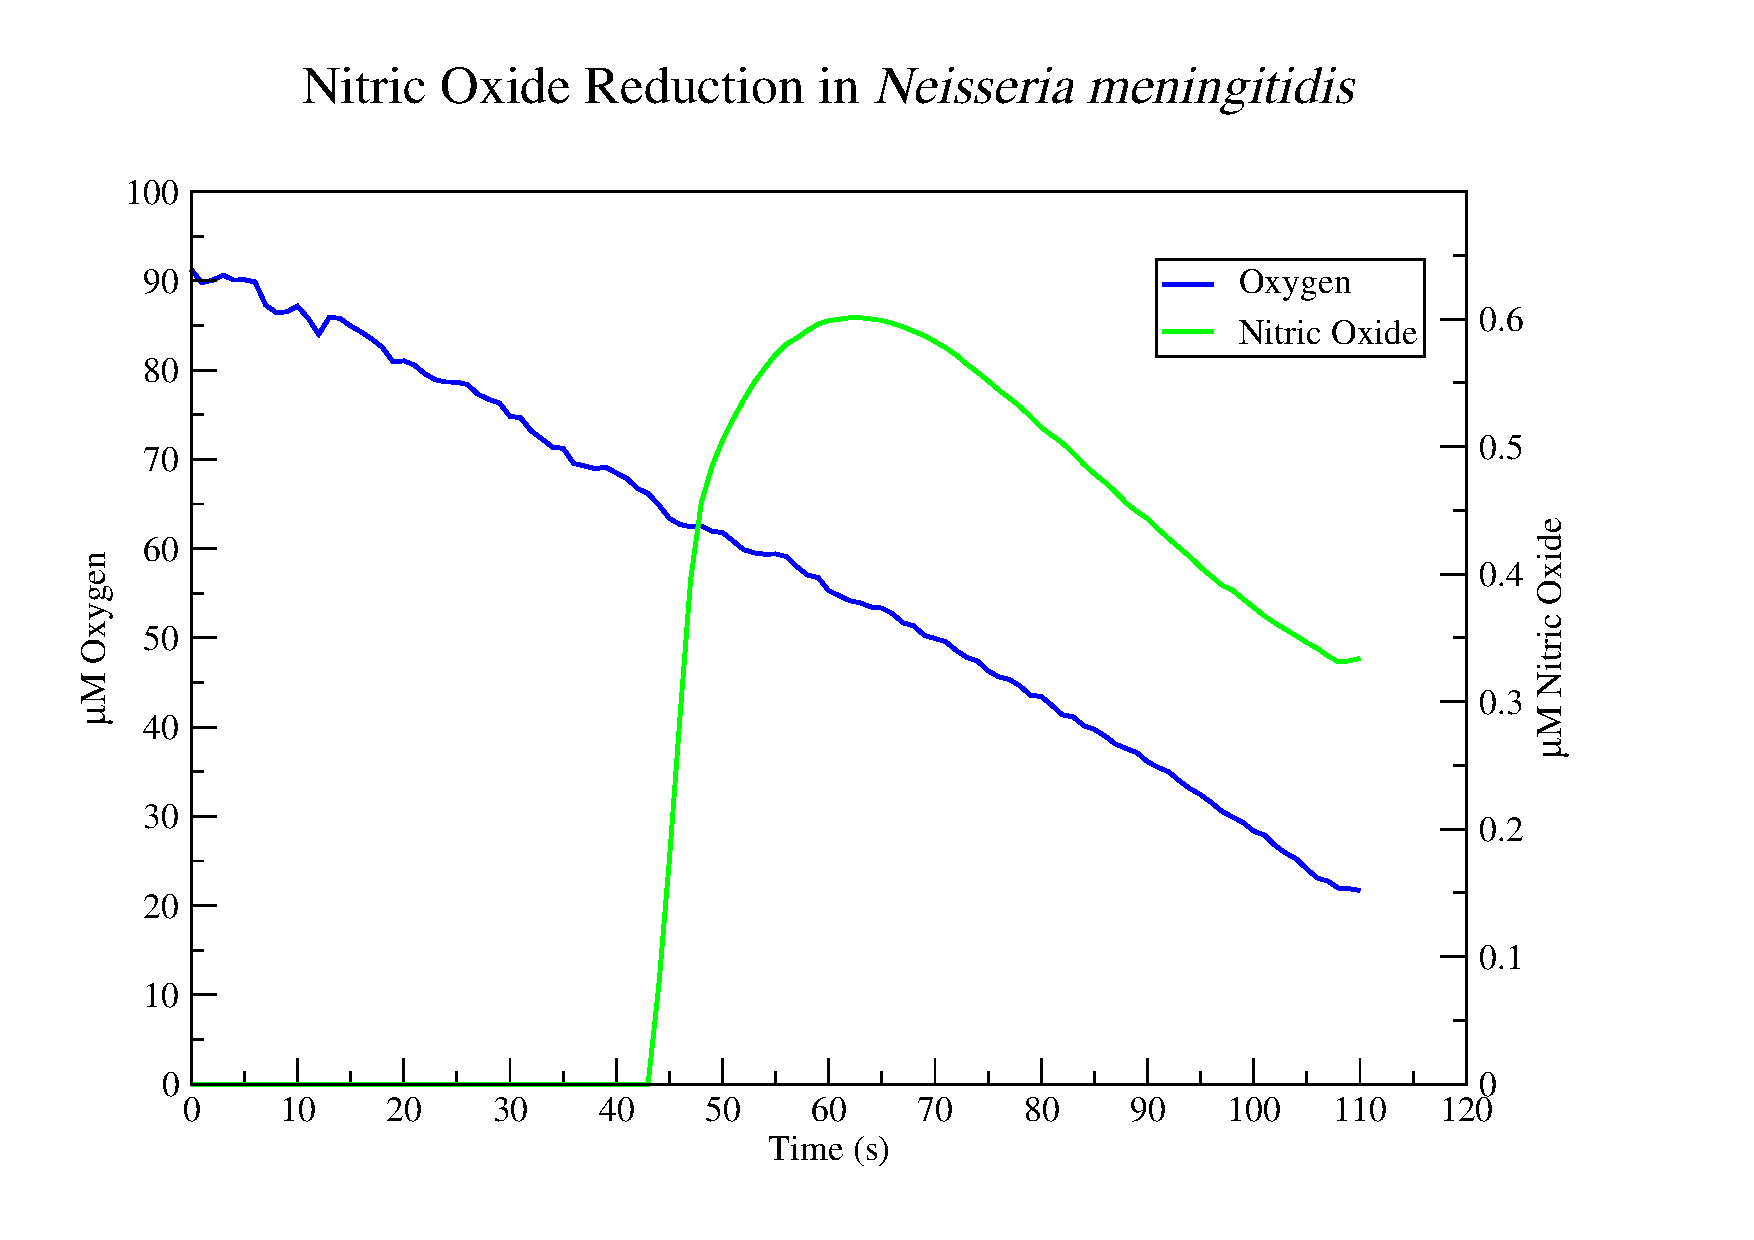
\includegraphics[height=10cm, trim=2cm 1cm 4cm 1cm]{./06-noreduction/data/aer-no-data1.pdf}
 % nosim.eps: 0x0 pixel, 300dpi, 0.00x0.00 cm, bb=0 0 794 595
 \caption[{Nitric Oxide Reduction in \textit{Neisseria meningitidis}.}]{{\bf Nitric Oxide Reduction in \textit{Neisseria meningitidis}.} This dataset shows the effect on rate of oxygen reduction as a small amount of nitric oxide (to $\approx 0.6~\mu M$) is introduced to the respiring system.}
 \label{fig:nodata1}
\end{figure}
The dataset in Figure \ref{fig:nodata1} shows very little visible change in the rate of oxygen reduction when a small amount of nitric oxide is added. In actual fact the change in rate was an $\approx 3\%$ reduction after addition of nitric oxide based on linear regression of pre- and post-addition rates. The observed removal of nitric oxide is due primarily to diffusion, although there may also be some preliminary (as the culture has not been primed with nitric oxide) nitric oxide reductase activity. However for modelling purposes it was assumed that the nitric oxide reductase activity for this dataset is zero.

\begin{figure}[tbp]
 \centering
 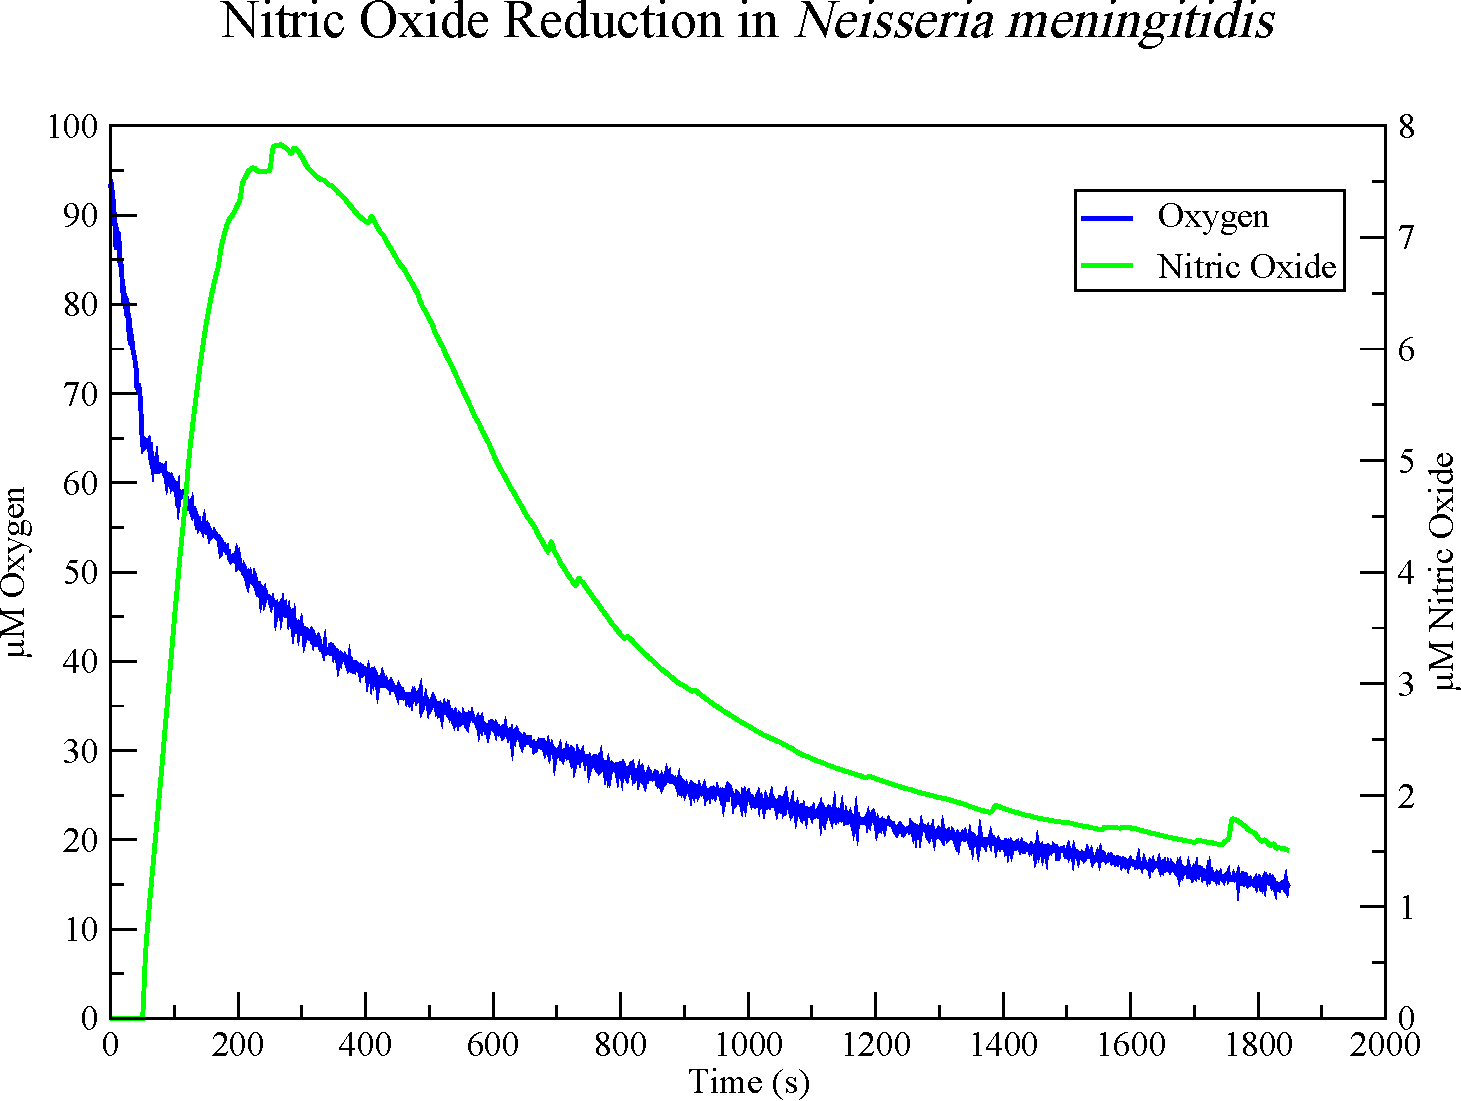
\includegraphics[height=10cm, trim=2cm 1cm 4cm 1cm]{./06-noreduction/data/aer-no-data2.pdf}
 % nosim.eps: 0x0 pixel, 300dpi, 0.00x0.00 cm, bb=0 0 794 595
 \caption[{Nitric Oxide Reduction in \textit{Neisseria meningitidis}.}]{{\bf Nitric Oxide Reduction in \textit{Neisseria meningitidis}.} This dataset shows the effect on rate of oxygen reduction as a larger amount of nitric oxide (to $\approx 7.8~\mu M$) is introduced to the respiring system.}
 \label{fig:nodata2}
\end{figure}
The dataset in Figure \ref{fig:nodata2} shows a larger change in the rate of oxygen reduction than that of Figure \ref{fig:nodata1} when a larger amount of nitric oxide is introduced. Again the removal of nitric oxide will primarily be due to diffusion, although now at higher concentrations more nitric oxide will interact with \cbbthree{} temporarily inhibiting it. This inhibition causes the reduction in oxidase activity, and the sequestering of NO by \cbbthree{} also causes some of the visible reduction in nitric oxide concentration. The time-scale over which the nitric oxide disappears strongly suggests that it is not due to nitric oxide reductase activity. It may also be possible that at this concentration of nitric oxide some \cbbthree{} may have been permanently inhibited as mentioned in Chapters \ref{chap:intro} \& \ref{chap:model}. As the cultures in this dataset were obviously being negatively affected by the addition of such a high concentration of nitric oxide, either by permanent inhibition of \cbbthree{} or actual cell death, it was unlikely that this particular dataset could be used to accurately predict parameters in the model as it includes factors that were never part of the original model.

\begin{figure}[tbp]
 \centering
 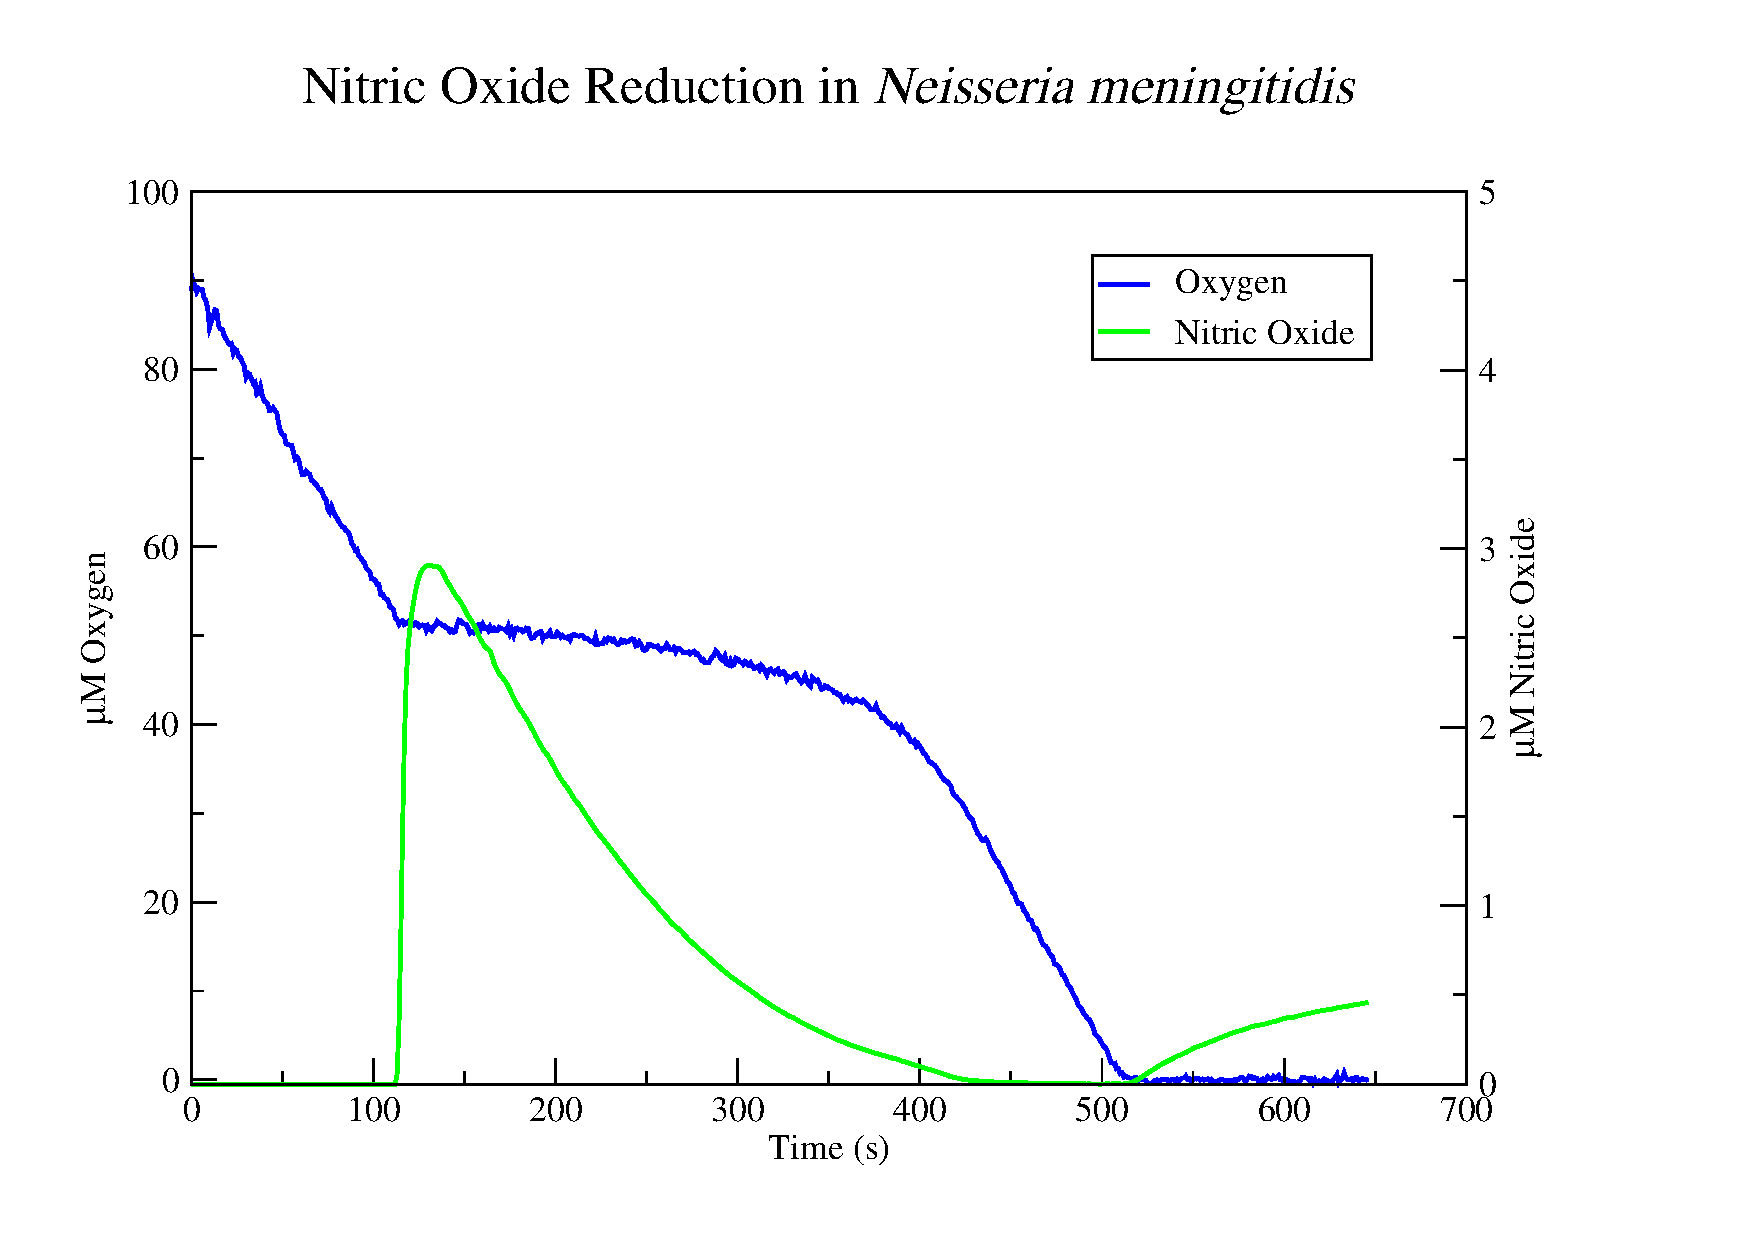
\includegraphics[height=10cm, trim=2cm 1cm 4cm 1cm]{./06-noreduction/data/aer-no-data.pdf}
 % nosim.eps: 0x0 pixel, 300dpi, 0.00x0.00 cm, bb=0 0 794 595
 \caption[{Nitric Oxide Reduction in \textit{Neisseria meningitidis}.}]{{\bf Nitric Oxide Reduction in \textit{Neisseria meningitidis}.} This dataset shows the effect on rate of oxygen reduction as nitric oxide (to $\approx 3~\mu M$) is introduced to respiring the system which also appears to have been partially primed for nitric oxide reduction.}
 \label{fig:nodata}
\end{figure}
The dataset in Figure \ref{fig:nodata} appears to show a system that was partially primed for microaerobic respiration. In this case it was speculated that there was a small amount of NorB (nitric oxide reductase) present. Initially the oxygen reduction was carried out in exactly the same manner as in Chapter \ref{chap:oxygenreduction}. Upon addition of nitric oxide, oxygen respiration slowed and almost stopped as a result of competition for electrons between \cbbthree{} and NorB, and the direct chemical inhibition of \cbbthree{} by NO. Nitric oxide started to be removed as a combination of diffusion (although this rate will be low as shown in the previous two datasets) and reduction via NorB. Once the NO has been removed from the system oxygen reduction resumes at almost the same rate as before and still has the same high affinity feature as the oxygen reduction datasets in Chapter \ref{chap:oxygenreduction}.
\subsubsection{Prior Probability Distributions}
As in Chapter \ref{chap:oxygenreduction} the integrative scheme requires that all the parameters involved have associated prior probability distributions. The posterior probability distributions from Chapter \ref{chap:oxygenreduction} were used as prior probability distributions in this chapter. Where new parameters were introduced (which had not been modelled thus far), the distributions were generated based upon published literature values which are noted in Chapter \ref{chap:model}. When using literature values the prior probability distributions were generated according to the same scheme as in Chapter \ref{chap:oxygenreduction}. Where the posterior probability distributions from Chapter \ref{chap:oxygenreduction} describe rate constants the raw values from the distributions were used as priors in this chapter. Where the distributions describe component concentrations, idealised lognormal distributions were used instead of the raw data to account for differing concentrations between cultures. The distribution of the parameter $\gamma$ - the rate of loss of NO - was initially assumed to be similar to $\beta$, thus the same probability distribution was used. For the other new parameters, lognormal distributions were used as priors as described in Chapter \ref{chap:oxygenreduction}. The values required to create idealised lognormal probability distributions for each parameter are shown in Table \ref{tab:noProbstat1}.

\begin{table}[ht]%needs to be 'here' as section is short
\renewcommand{\arraystretch}{1.5}
\begin{center}
\begin{tabular}{cccc|cccc}
\toprule
\textbf{Parameter} && ${\bar{x}}$ & $\sigma$ & \textbf{Parameter} && ${\bar{x}}$ & $\sigma$\\
\midrule
$k_1$ && 450 & 35 & $\gamma$ && 0.00014 & $4.72\times 10^{-6}$\\
$k_3$ && 4.748 & 0.404 & Q && 3.59 & 0.132\\
$l_1$ && 6 & 2 & X && 15.177 & 0.247\\
$l_3$ && 1 & 2 & B && 0.143 & 0.159\\
$k_5$ && 100 & 10 & C && 0.143 & 0.159\\
$k_6$ && 38 & 8 & $Q_a$ && 0.24 & 0.034\\
$\beta$ && 0.00014 & $4.72\times 10^{-6}$ & $X_a$ && 3.176 & 0.039\\
g && 1.053 & 0.099 & $B_a$ && 0.024 & 0.036\\
f && 9.10 & 1.18 & $C_a$ && 0.024 & 0.036\\
\bottomrule
\end{tabular}
\end{center}
\caption[Prior Probability Table]{{\bf Prior Probability Table} This table shows the prior means and standard deviations used to create lognormal distributions to be used as the prior probability distributions.
\label{tab:noProbstat1}}
\end{table}
\afterpage{\clearpage}
The initial probability distributions used to start the Monte-Carlo runs are shown in Figure \ref{fig:aer_no_priors}.
\begin{figure}[tbp]
 \centering
 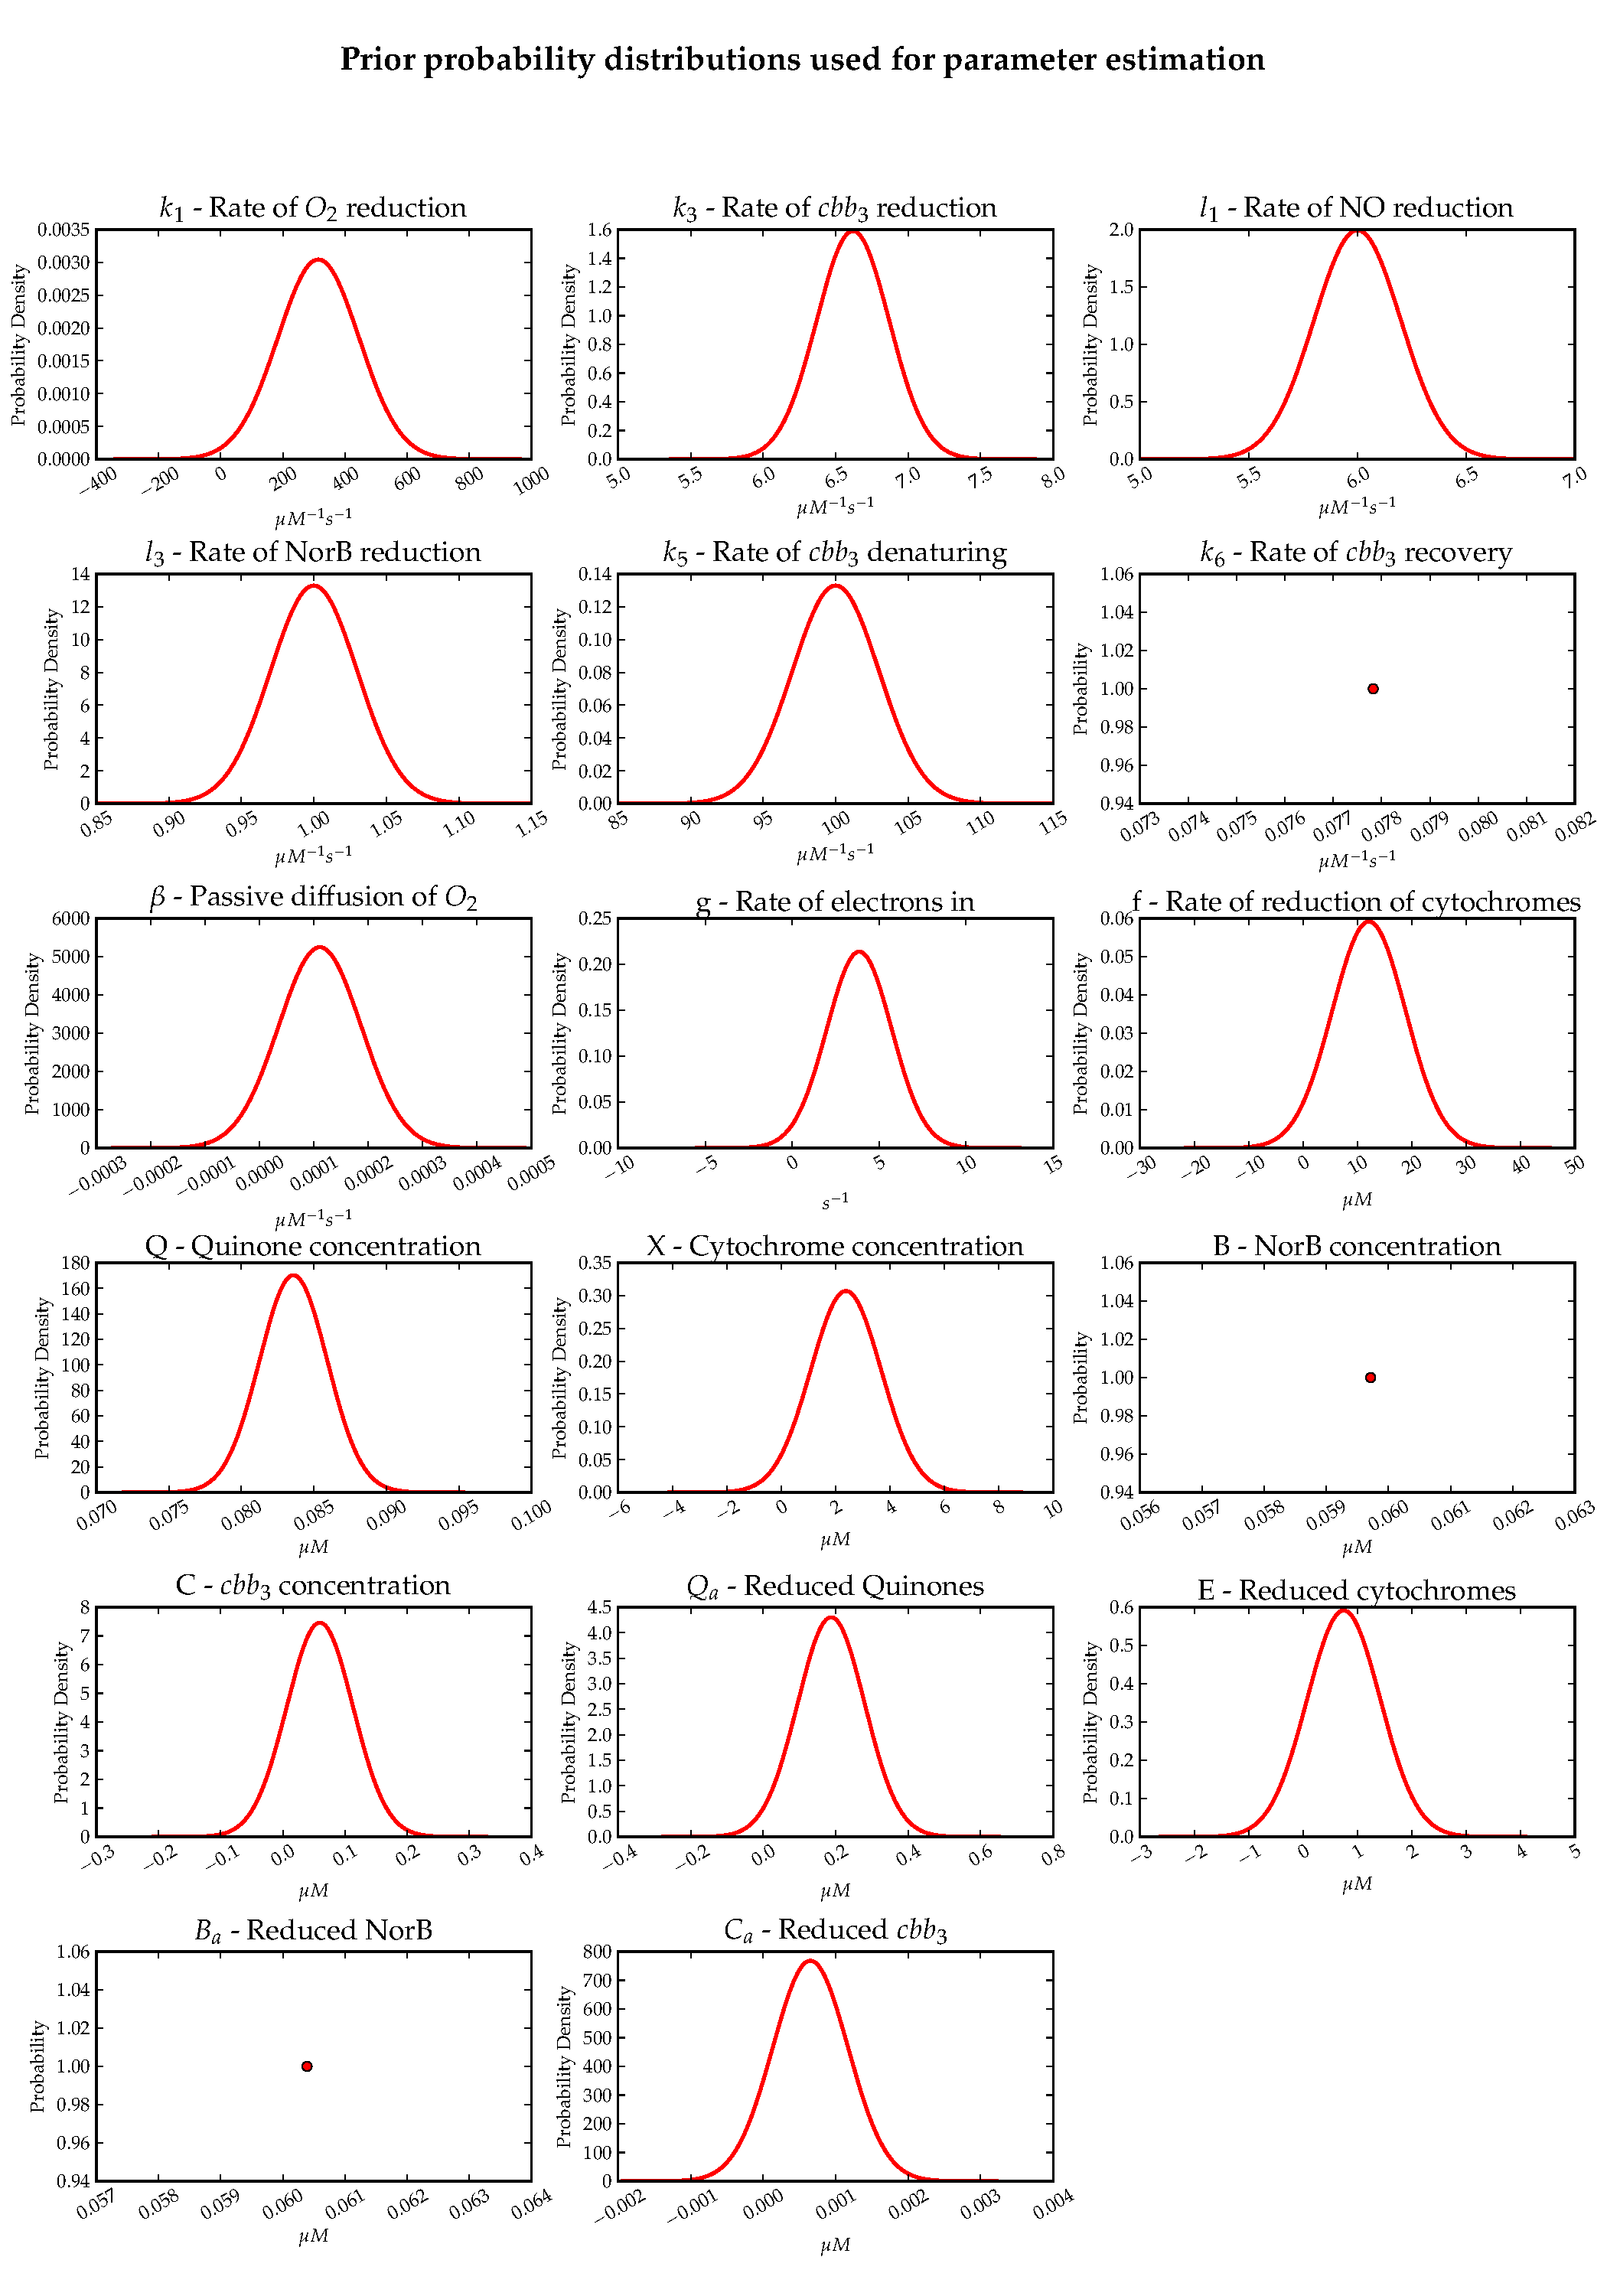
\includegraphics[width=15cm, trim=0cm 0cm 0cm 0cm]{./06-noreduction/data/aer-no-priors.pdf}
 % priors.pdf: 1008x1008 pixel, 72dpi, 35.56x35.56 cm, bb=0 0 1008 1008
 \caption[Prior probability distributions for aerobic nitric oxide reduction]{{\bf Prior probability distributions for aerobic nitric oxide reduction}. These are the probability distributions used as priors by the parameter estimation algorithm.
 \label{fig:aer_no_priors}}
\end{figure}

\subsubsection{Parameter Estimation Results}
The parameter estimation process was run in the same fashion as that described in Chapter \ref{chap:oxygenreduction}. The 3 experimental datasets were run 20 times (each) for 20,000 iterations using the prior probability distributions shown in Figure \ref{fig:aer_no_priors}. This generated parameter trajectories from each of the 3 datasets. The second dataset was still analysed even though it is unlikely that the model will successfully be able to be parametrised from it. Unfortunately upon examination of the \textit{BOF} values from the MHMC output and the best-fitting solved output it was clear that the prior probability distributions in conjunction with the model are incapable of accurately describing the experimental data. This strongly suggested that the new prior probability distributions (those obtained from the literature for the NO related components) were incorrect.

The result from dataset 3

%A representative example of the solved output from one of the trajectories from the experimental dataset shown in Figure \ref{fig:nodata} is shown in Figure \ref{fig:nosim}. This figure was generated from the set of parameters that produced the most fit output compared to the input dataset.
%\begin{figure}[tbp]
% \centering
% 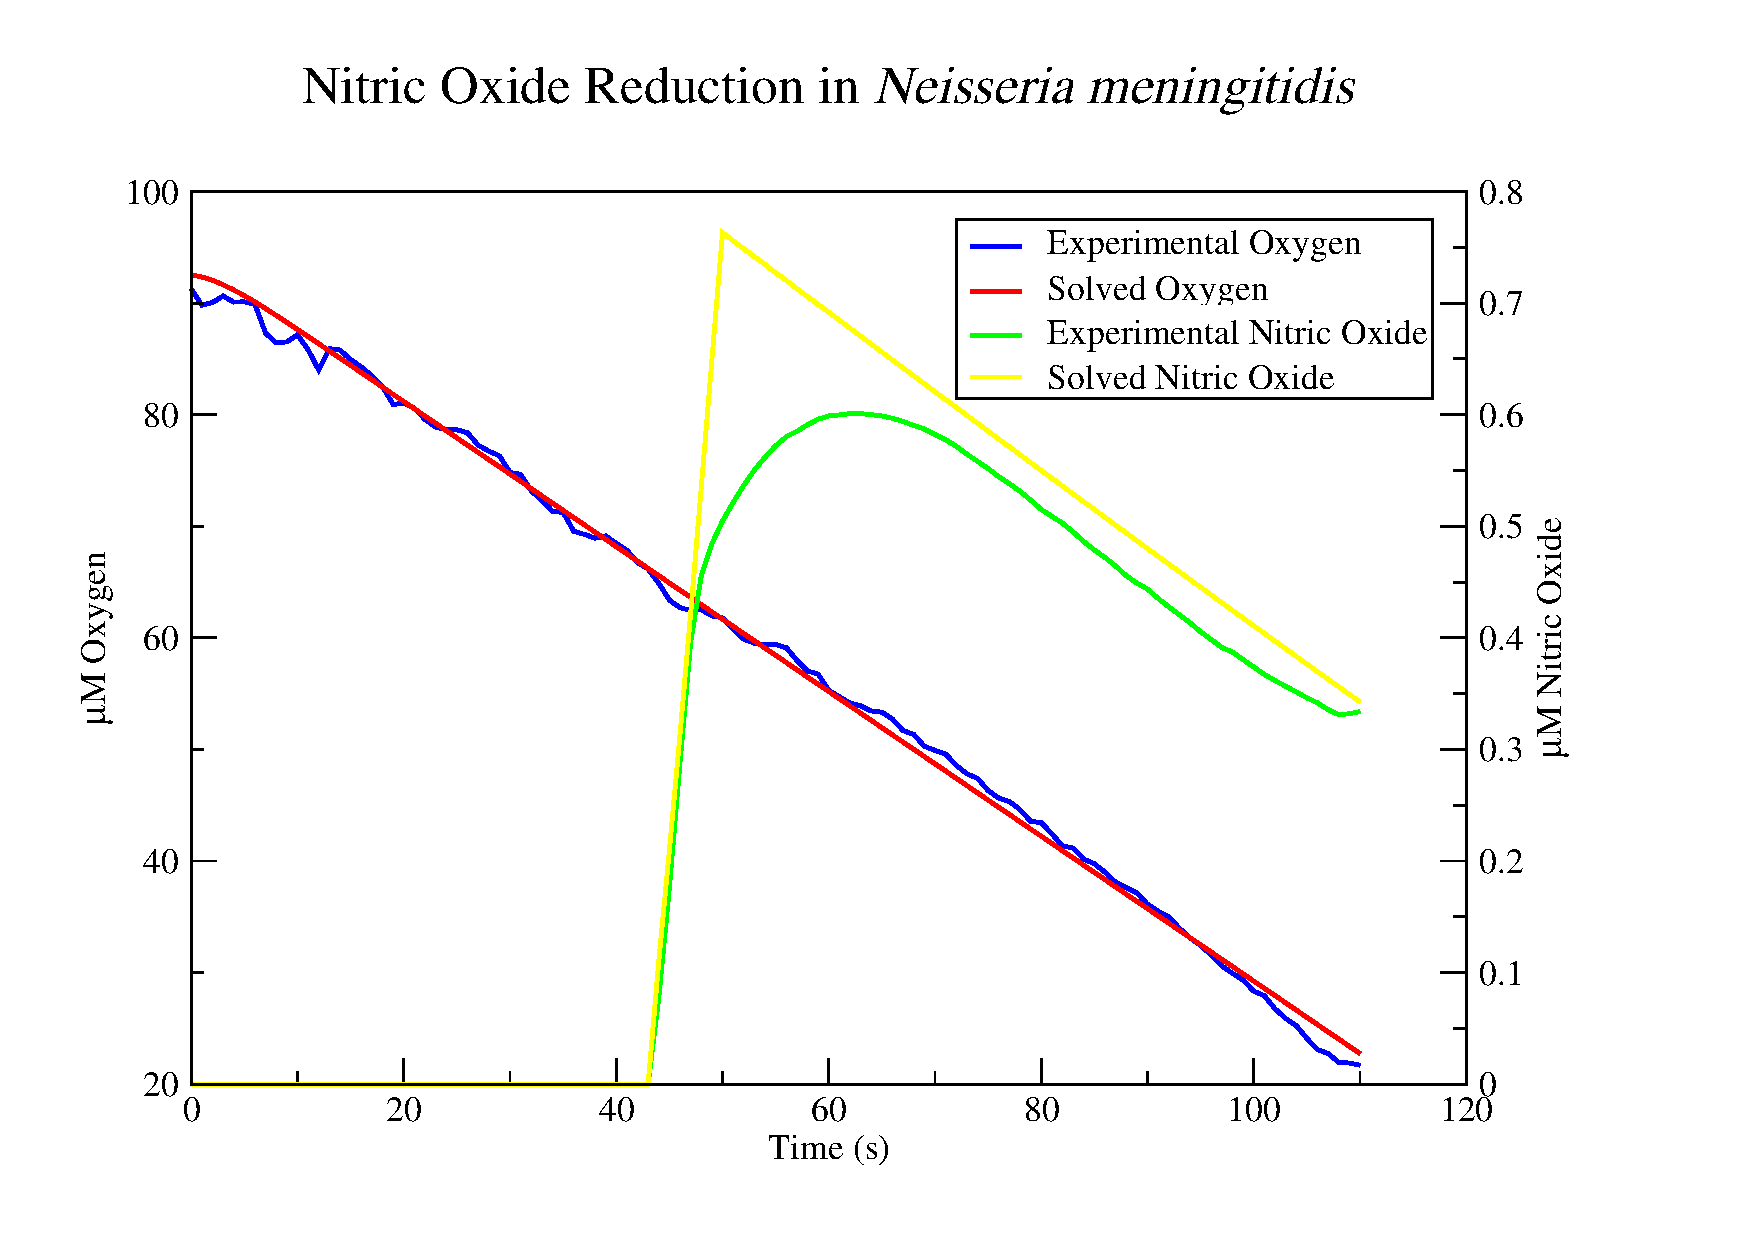
\includegraphics[width=14cm, trim=1cm 1cm 3cm 1cm, clip=true]{./06-noreduction/data/aer-no-sim1.pdf}
% % nosim.eps: 0x0 pixel, 300dpi, 0.00x0.00 cm, bb=0 0 794 595
% \caption[{Nitric Oxide Reduction in \textit{Neisseria meningitidis}.}]{{\bf Nitric Oxide Reduction in \textit{Neisseria meningitidis}.} This dataset shows the effect on rate of oxygen reduction as nitric oxide is introduced to the system. The solved output, using prior probabilities from the oxygen reduction dataset show an almost perfect match to the features of the experimental dataset.}
% \label{fig:nosim}
%\end{figure}
%The model was able to generate a parameter set from the prior probability distributions that could accommodate all the new features of the dataset as evidenced by the closeness of fit of the solved output to the experimental data. This parameter set will also still be able to model simple oxygen reduction.
\subsubsection{Analysis of Convergence}
\subsubsection{Analysis of Correlation}
\begin{table}[p]
\setlength{\tabcolsep}{5pt}
\renewcommand{\arraystretch}{1.5}
  \centering
  \rotatebox{90}{
  \begin{minipage}{24.4cm}
  \centering
  \begin{tabular}{|c|c|c|c|c|c|c|c|c|c|}
    \hline
    \cellcolor{dark-gray} & \cellcolor{dark-gray}$k_1$ & \cellcolor{dark-gray}$k_3$ & \cellcolor{dark-gray}$\beta$ & \cellcolor{dark-gray}g & \cellcolor{dark-gray}f & \cellcolor{dark-gray}Q & \cellcolor{dark-gray}X & \cellcolor{dark-gray}C \\
    \hline
    \cellcolor{dark-gray}$k_1$ & \cellcolor{light-gray}$1$ & 0.009239 & 0.017156 & 0.049769 & -0.011922 & 0.020906 & 0.022824 & 0.033631 \\
    \hline
    \cellcolor{dark-gray}$k_3$ & \cellcolor{light-gray} & \cellcolor{light-gray}$1$ & -0.027037 & -0.083623 & 0.052659 & -0.040318 & -0.202936 & \cellcolor{orange}-0.411031 \\
    \hline
    \cellcolor{dark-gray}$\beta$ & \cellcolor{light-gray} & \cellcolor{light-gray} & \cellcolor{light-gray}$1$ & -0.002919 & 0.000809 & -0.013785 & 0.007012 & 0.022641 \\
    \hline
    \cellcolor{dark-gray}g & \cellcolor{light-gray} & \cellcolor{light-gray} & \cellcolor{light-gray} & \cellcolor{light-gray}$1$ & -0.038259 & \cellcolor{orange}-0.332178 & 0.199383 & -0.152613 \\
    \hline
    \cellcolor{dark-gray}f & \cellcolor{light-gray} & \cellcolor{light-gray} & \cellcolor{light-gray} & \cellcolor{light-gray} & \cellcolor{light-gray}$1$ & -0.03624 & -0.087711 & -0.034303 \\
    \hline
    \cellcolor{dark-gray}Q & \cellcolor{light-gray} & \cellcolor{light-gray} & \cellcolor{light-gray} & \cellcolor{light-gray} & \cellcolor{light-gray} & \cellcolor{light-gray}$1$ & 0.083179 & -0.043061 \\
    \hline
    \cellcolor{dark-gray}X & \cellcolor{light-gray} & \cellcolor{light-gray} & \cellcolor{light-gray} & \cellcolor{light-gray} & \cellcolor{light-gray} & \cellcolor{light-gray} & \cellcolor{light-gray}$1$ & \cellcolor{orange}-0.577183 \\
    \hline
    \cellcolor{dark-gray}C & \cellcolor{light-gray} & \cellcolor{light-gray} & \cellcolor{light-gray} & \cellcolor{light-gray} & \cellcolor{light-gray} & \cellcolor{light-gray} & \cellcolor{light-gray} & \cellcolor{light-gray}$1$ \\
    \hline
  \end{tabular}
  \caption[Regression Analysis of Oxygen Reduction Parameters]{{\bf Regression Analysis of Oxygen Reduction Parameters for Dataset 2.} This table shows the $R$ values from linear regression analysis on the combined parameter trajectories for Oxygen reduction. Parameters with high correlation have been coloured green ($R>0.8$) and those with moderation correlation have been coloured orange ($0.8>R>0.3$).
  \label{tab:noregress1}}
  \end{minipage}
  }
\end{table}
\afterpage{\clearpage}
%\end{landscape}
\begin{table}[p]
\setlength{\tabcolsep}{5pt}
\renewcommand{\arraystretch}{1.5}
  \centering
  \rotatebox{90}{
  \begin{minipage}{24.4cm}
  \centering
  \begin{tabular}{|c|c|c|c|c|c|c|c|c|c|}
    \hline
    \cellcolor{dark-gray} & \cellcolor{dark-gray}$k_1$ & \cellcolor{dark-gray}$k_3$ & \cellcolor{dark-gray}$\beta$ & \cellcolor{dark-gray}g & \cellcolor{dark-gray}f & \cellcolor{dark-gray}Q & \cellcolor{dark-gray}X & \cellcolor{dark-gray}C \\
    \hline
    \cellcolor{dark-gray}$k_1$ & \cellcolor{light-gray}$1$ &0.06739 & 0.005008 & 0.222959 & -0.077916 & -0.243691 & 0.056941 & -0.036059 \\
    \hline
    \cellcolor{dark-gray}$k_3$ & \cellcolor{light-gray} & \cellcolor{light-gray}$1$ & 0.249 & -0.173314 & \cellcolor{orange}0.304448 & 0.018672 & \cellcolor{orange}-0.487193 & \cellcolor{orange}-0.313064 \\
    \hline
    \cellcolor{dark-gray}$\beta$ & \cellcolor{light-gray} & \cellcolor{light-gray} & \cellcolor{light-gray}$1$ & 0.065203 & -0.033434 & 0.053464 & -0.026229 & -0.174494 \\
    \hline
    \cellcolor{dark-gray}g & \cellcolor{light-gray} & \cellcolor{light-gray} & \cellcolor{light-gray} & \cellcolor{light-gray}$1$ & -0.276682 & -0.104876 & 0.250671 & -0.210795 \\
    \hline
    \cellcolor{dark-gray}f & \cellcolor{light-gray} & \cellcolor{light-gray} & \cellcolor{light-gray} & \cellcolor{light-gray} & \cellcolor{light-gray}$1$ & -0.146998 & \cellcolor{orange}-0.496387 & 0.243878 \\
    \hline
    \cellcolor{dark-gray}Q & \cellcolor{light-gray} & \cellcolor{light-gray} & \cellcolor{light-gray} & \cellcolor{light-gray} & \cellcolor{light-gray} & \cellcolor{light-gray}$1$ & 0.158161 & \cellcolor{orange}-0.397437 \\
    \hline
    \cellcolor{dark-gray}X & \cellcolor{light-gray} & \cellcolor{light-gray} & \cellcolor{light-gray} & \cellcolor{light-gray} & \cellcolor{light-gray} & \cellcolor{light-gray} & \cellcolor{light-gray}$1$ & \cellcolor{orange}-0.624574 \\
    \hline
    \cellcolor{dark-gray}C & \cellcolor{light-gray} & \cellcolor{light-gray} & \cellcolor{light-gray} & \cellcolor{light-gray} & \cellcolor{light-gray} & \cellcolor{light-gray} & \cellcolor{light-gray} & \cellcolor{light-gray}$1$ \\
    \hline
  \end{tabular}
  \caption[Regression Analysis of Oxygen Reduction Parameters]{{\bf Regression Analysis of Oxygen Reduction Parameters for Dataset 3.} This table shows the $R$ values from linear regression analysis on the combined parameter trajectories for Oxygen reduction. Parameters with high correlation have been coloured green ($R>0.8$) and those with moderation correlation have been coloured orange ($0.8>R>0.3$).
  \label{tab:noregress2}}
  \end{minipage}
  }
\end{table}
\afterpage{\clearpage}
\subsection{Discussion}
\section{Microaerobic Nitric Oxide Reduction}
\subsection{Introduction}
\subsection{Results}
\subsection{Discussion}
\section{\texorpdfstring{Aerobic Nitric Oxide Reduction in \textit{nsrR$^\textrm{-}$} mutant}{Aerobic Nitric Oxide Reduction in nsrR- mutant}}
\subsection{Introduction}
 The $\mathit{nsrR}^-$ mutant, which expresses NorB in an essentially constitutive manner was not effective in generating a usable dataset as it removed any NO almost instantaneously resulting in an almost featureless dataset (data not shown).
\subsection{Results}
\subsection{Discussion}